% !TEX encoding = UTF-8 Unicode
\documentclass[a4paper]{report}
\usepackage{tikz}
\usepackage[margin=2.5cm]{geometry}
\usepackage{hyperref}
\usepackage{graphicx}
\usepackage{parskip}
\graphicspath{{figures/}{anotherFigureDirectory/}}
\graphicspath{ {./images/} }
\usepackage{listings}
\usepackage{wrapfig}
\usepackage{float}
\usepackage{color}
\definecolor{bluekeywords}{rgb}{0.13,0.13,1}
\definecolor{greencomments}{rgb}{0,0.5,0}
\definecolor{turqusnumbers}{rgb}{0.17,0.57,0.69}
\definecolor{redstrings}{rgb}{0.5,0,0}
\definecolor{gray}{rgb}{0.13,0.13,0.13}
\lstdefinelanguage{FSharp}
                {morekeywords={let, new, match, with, rec, open, module,
                namespace, type, of, member, and, for, in, do, begin, end, fun,
                function, try, mutable, if, then, else},
                keywordstyle=\color{bluekeywords},
                sensitive=false,
                numbers=left,  % where to put the line-numbers;(none, left, right)
                numberstyle=\tiny\color{gray},
                morecomment=[l][\color{greencomments}]{///},
                morecomment=[l][\color{greencomments}]{//},
                morecomment=[s][\color{greencomments}]{{(*}{*)}},
                morestring=[b]",
                showstringspaces=false,
                stringstyle=\color{redstrings}
                }

\title{PoP - Ugeopgave 10}
\author{Christoffer, Inge og Pernille}
\date{\today}

\begin{document}
\maketitle
\tikzstyle{block} = [rectangle, draw, fill=blue!20, text centered,
    rounded corners, minimum height=2.5em]
\tikzstyle{cloud} = [rectangle, draw, fill=white, text centered,
    rounded corners, minimum height = 2em]
\tikzstyle{line} = [draw, -latex]




\section*{Preface}
As our first semester course in Programming and Problem Solving has entered a new programming paradigm, namely object oriented (OO) programming, we, three budding computer scientists have build a small environment based on the small island Isle Royale. We've used the multi paradigm programming language Fsharp (F\#), to code our entire OO environment.

\section*{Introduction}
Isle Royale is a small desolate island located in Lake Superior split by the North America-Canadian border. The island is inhabited by wolves and moose. The population of the two mammals, predator and prey have shown over time to be highly interdependent.
Through no less than 5 decades the research project "Wolves and Moose of Isle Royale" has monitored the lives and deaths of the animals of the island, making \textit{"the longest continuous study of any predator-prey system in the world."} \url{(http://www.isleroyalewolf.org/overview/overview/at_a_glance.html)}



\section*{Problem analysis \& design}
As given by the assignment, the entire Isle Royale environment is implemented in f\# by use of the object oriented programming paradigm.

The main task of the assignment was to simulate the flow and development of the animal population of Isle Royale in an enclosed environment.

From the offset of the assignment, we we're given an unfinished library and a corresponding signaturefile.
Here we we're given an extended part of the code, which needed to be built in order to meet the assignment criteria.
This included an animal object, moose object (unfinished), wolf object (unfinished) and an object for the environment of the isle (also unfinished).

\begin{figure}[H]
\centering
\begin{tikzpicture} [node distance = 1.5 cm, auto]
		\node [cloud] (start) {New environment is created};
        \node [cloud, below of=start] (tick) {Tick};
        \node [cloud, right of=tick, node distance = 5 cm]
            (moose) {Moose};
        \node [cloud, below of=moose, node distance = 3 cm]
            (mlive) {Live};
        \node [cloud, left of=mlive, node distance = 3 cm]
            (eaten) {Eaten by wolf}; 
        \node [cloud, below of=mlive, node distance = 3 cm]
            (mgiveb) {Give birth};
        \node [cloud, right of=mlive, node distance = 3 cm]
            (movem) {New position}; 
		\node [cloud, left of=tick, node distance = 5 cm]
            (wolf) {Wolf};
        \node [cloud, left of=wolf, node distance = 3 cm]
            (die) {Die};
        \node [cloud, below of=wolf, node distance = 3 cm]
            (wlive) {Live};
        \node [cloud, left of=wlive, node distance = 3 cm]
            (eat) {Eats moose}; 
        \node [cloud, below of=wlive, node distance = 3 cm]
            (wgiveb) {Give birth};
        \node [cloud, right of=wlive, node distance = 3 cm]
            (movew) {New position}; 
            
        % Arrows
        \path [line] (start) -- (tick);
        \path [line] (tick) -- (wolf);
        \path [line] (tick) -- (moose);
        \path [line] (wolf) -- (die);
        \path [line] (wolf) -- (wlive);
        \path [line] (moose) -- (mlive);
        \path [line] (mlive) -- (eaten);
        \path [line] (mlive) -- (movem);
        \path [line] (mlive) -- (mgiveb);
        \path [line] (wlive) -- (eat);
        \path [line] (wlive) -- (movew);
        \path [line] (wlive) -- (wgiveb);
\end{tikzpicture}
\caption{Flow of Isle Royale environment}
\label{fig:gameflow}
\end{figure}


\subsection*{Environment}
The enviroment includes a board. The board consists of a width and two lists of animals. In environment, there are several crucial functions that deals with the problems of updating the animals and drawing the board, e.g. \texttt{updateMoose}, \texttt{updateWolf}, \texttt{draw}  and \texttt{tick}.

\subsubsection*{Ticks}
The method \texttt{tick} calls the function \texttt{procesLists} that updates different entities, as mentioned. So every time a tick is called, the environment at the board is updated. Thereby, tick functions as a time unity and every time a tick is called, we can imagine that a month or perhaps a week has passed. At Figure 1, we see that the \texttt{tick} has a central position that activates updates for the animals.

\subsubsection*{Moose}
The Moose object is created to live a simple life, so to speak. Aside from the fields and members inherited from the animal object, it's methods consists of just two members: One enabling reproduction and one handling the update of the reproduction and thereby the potential birth of a calf.

\subsubsection*{Wolwes}
The wolf object also inherits all fields and members of the animal object. The wolf, as the Moose, can reproduce and give birth to a cub in order to increase the population of wolfs on the island. Moreover the wolf can eat a moose populating a nearby position in the environment. 

\subsection*{Program description}

The environment is handling the animals and drawing the board. The main function in environment is \texttt{processLists}  as it is the only functions called when the method tick is called.
\texttt{processLists} selects an animal passes it on to one of the two helper functions called \texttt{handleMoose}  and \texttt{handleWolf}. In those any dead animals are removed from the board and the selected animal is passed further on to the one of the two functions \texttt{updateMoose} and \texttt{updateWolf}. The \texttt{updateMoose} function is responsible for the moose either giving birth or moving to a new position.
The \texttt{updateWolf} function does the same, but also has the added capability of making the wolf eat a moose if any is located in one of the neighbouring coordinates.

\subsubsection*{processList}
\texttt{processLists} is shown below. It gets a wolves list and a moose list as input and remove dead animals from them in \texttt{handleWolf} and \texttt{handleMoose}. Via a match, it then processes those lists.

\lstinputlisting[language=FSharp, firstline=222, lastline=247]{animalsSmall.fs}

\subsubsection*{checkNabour}
The check \texttt{checkNabour} function returns a list with the neighbouring coordinates and their symbols. The update functions use it to find out whether the wolf should eat a moose, give birth or move by checking for moose or empty symbols.


\lstinputlisting[language=FSharp, firstline=121, lastline=136]{animalsSmall.fs}

\subsubsection*{updateWolf}


The code from \texttt{updateWolf} is below. First is udates a tick to see whether the wolf has died. Then it looks for a moose in the neighbour position to find out whether it should eat. If so, the wolf eats the moose and goes to the moose' position. If it is not so, the function looks for an empty position if a cub is born, so that it can give birth to it by giving the cub a position. Else, it moves to that position itself. 

As mentioned, \texttt{updateMoose} is very similar, but shorter. Therefore it is not shown here.

\lstinputlisting[language=FSharp, firstline=178, lastline=209]{animalsSmall.fs}


\subsection*{Test}

Seeing as we were given a substantial code base created by our professor Jon Sporring, we were left with a limited amount of functions, which required testing.
Our first challenge in testing our own contribution to the code, was how to access local functions in the scope of classes and members, from outside “their”git  class, as it is standard in object oriented programming, that local functions are not editable nor accessible from outside their ambient scope.
To solve this, we chose to create members, within the scope of the respective class, which thereby had access to the given function. This way we were able to access and test the functions from a dedicated test file.
In all we’ve tested the following functions, which are all described in the section Program description:
\begin{itemize}
\item \texttt{checkNabour}
\item \texttt{updateMoose}
\item \texttt{updateWolf}
\item \texttt{processLists}
\end{itemize}

We also did an initial test of the \texttt{board} function, which mainly served as a pilot test of our general method for testing local functions.

\subsubsection{Test of \texttt{checkNabour}}
In the test of the \texttt{checkNabour} function, we tested with both a Moose and Wolf as animal input. On each animal object we did a run of 3 coherent calls to the function on the same randomly picked moose and wolf respectively, thereby disclosing a variety of function outputs, showing that the given animal does infect change position on the board, as the surrounding coordinates sometimes changes, and sometimes stays the same, in the case of the animal giving birth to a calf/cup.

\subsubsection{Test of \texttt{updateMoose} \&  \texttt{updateWolf}}
As with the test of  \texttt{checkNabour}, when testing \texttt{updateMoose} and  \texttt{updateWolf} we did a series of coherent calls to the function on a randomly picked moose and wolf. Again this shows how the position and reproduction length is updated as well as the hunger length, when testing the \texttt{updateWolf}. We see how the position coordinates and reproduction and hunger values change or remain the same, depending on whether a wolf eats or whether either of the animals give birth, thereby does not move and in which case their reproduction length is reset to it’s initial value. 

\subsubsection{Test of \texttt{processLists}}
Testing of the \texttt{processLists} function results in the least exiting result, as the output of a successful run of this function in any case will result in \texttt{<null>}, when running the function 
independent of the rest of the IsleRoyale program.

\subsection*{Experiments}
We have simulated three interesting experiments. One about hunger length, one about the size of the board and one about reproduction length. Small changes of the values shows a significant effect at the results. 

\subsubsection*{Board size}
The following comparison is about board width. If the board is large, as on Figure 2 where it is 40 X 40, the number of animals becomes rather large and the moose and the wolves co-exist throughout at least 80 ticks. 

\begin{figure}[H]
\centering
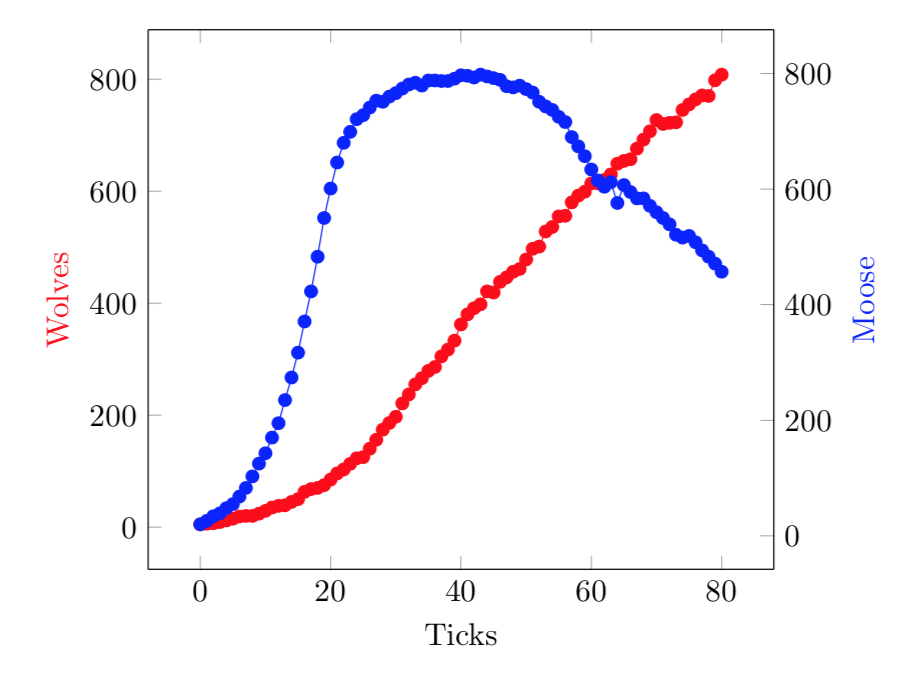
\includegraphics[width=0.60\textwidth]{Experiments/sim_board_b1}
\caption{Input values: ticks: 80, board width: 40, moose: 20, moose rep-length: 5, wolves: 5, wolf rep-length: 5, wolf hunger length: 8}
\end{figure}

Figure 3 represent a simulated environment where the board is only 20 X 20. Here, the number of moose becomes approximately 250 at tick 20 while it is 600 at the larger board in Figure 2. The same difference can be observed with the wolves. Another interesting observation is that the moose are extinct at tick 50 - whey get eaten by the wolves in the small amount of space. 

\begin{figure}[H]
\centering
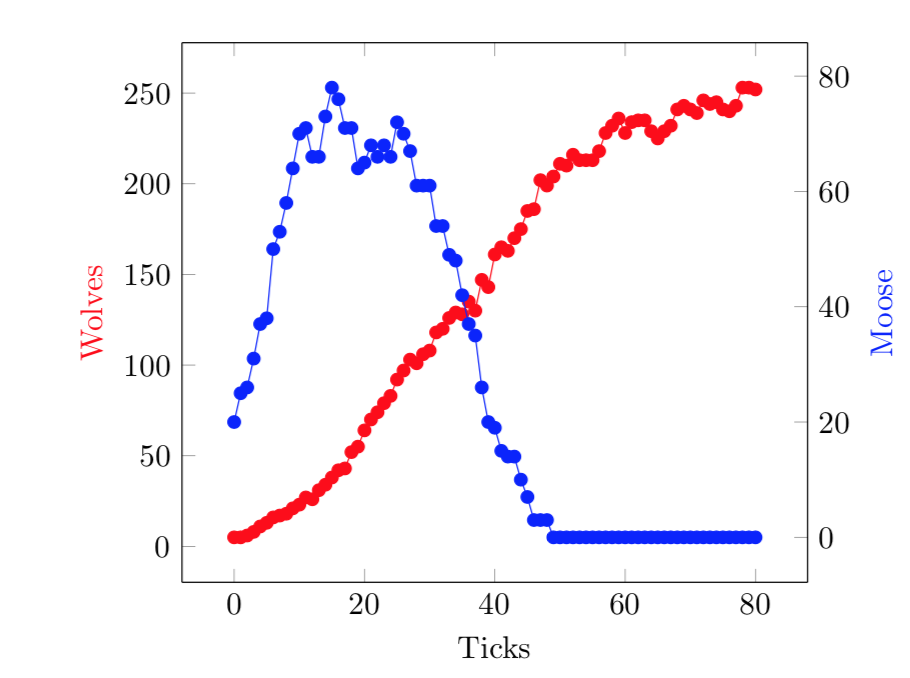
\includegraphics[width=0.60\textwidth]{Experiments/sim_board_b2} 
\caption{Input values: ticks: 80, board width: 20, moose: 20, moose rep-length: 5, wolves: 5, wolf rep-length: 5, wolf hunger length: 8}
\end{figure}

\subsubsection*{Hunger length}

Another experiment we have conducted focuses on the hunger length of the wolves. At Figure 4, the hunger length is rather shot, it is set to 4, so after 4 ticks the wolf will either die or have found a moose to eat. The result is, that only after 10 ticks the wolves are extinct while the moose keeps to increase in number.

\begin{figure}[H]
\centering
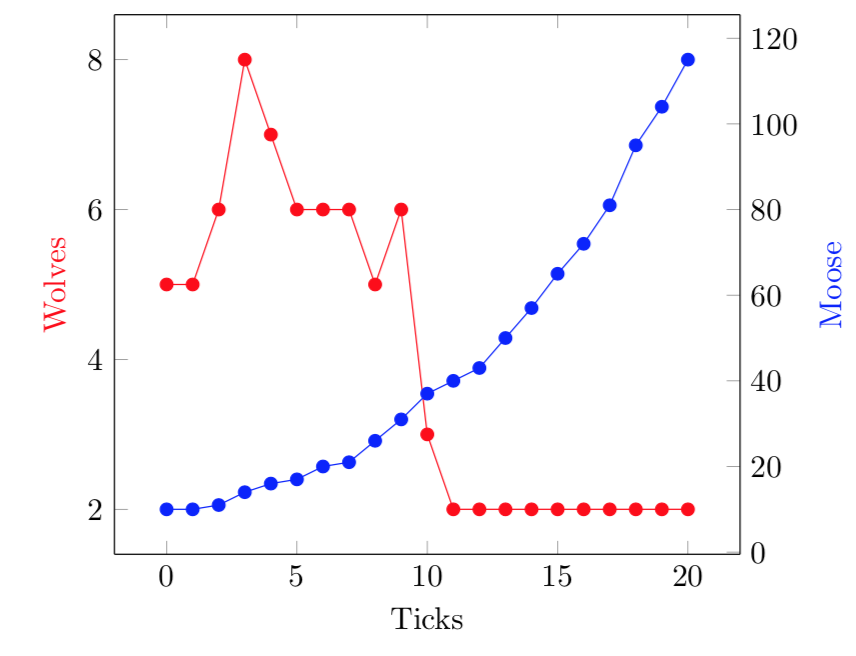
\includegraphics[width=0.60\textwidth]{Experiments/sim_hunlen_a1}
\caption{Input values: ticks: 20, board width: 15, moose: 10, moose rep-length: 5, wolves: 5, wolf rep-length: 5, wolf hunger length: 4}
\end{figure}

When we change the hunger length from 4 to 6 we get another result. As shown in the graph at Figure 5 we see that wolves does not extinct any more, but the moose does instead. At the beginning, the moose increase in number but around tick 10 the amount of wolves are so high that the number of moose start to decrease and at tick 16 they are all dead.

When the hunger length of the wolves is at 6, the wolves can exist for longer without eating. As the reproduction level is smaller than the hunger length, the wolf reproduce itself before it dies, and therefore they cannot extinct in this experiment, even if there are no moose left in the environment. Obviously, this means we should be conscious about the relation between the reproduction and the hunger length.

\begin{figure}[H]
\centering
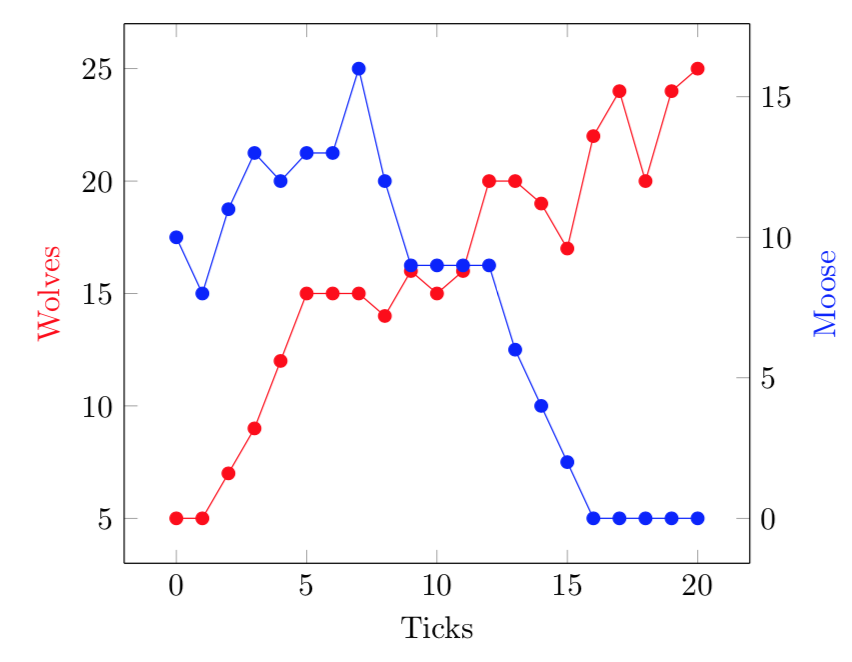
\includegraphics[width=0.60\textwidth]{Experiments/sim_hunlen_a2}
\caption{Input values: ticks: 20, board width: 15, moose: 10, moose reproduction length: 5, wolves: 5, wolf reproduction length: 5, wolf hunger length: 6}
\end{figure}


\subsubsection*{Reproduction length}
At Figure 6 and Figure 7 we see an experiment with variation in reproduction length. At Figure 6, the moose and the wolves have a longer reproduction length than on Figure 7. In both cases the number of moose increase rapidly within the first 20 ticks and then it stagnates.
 
At Figure 6, we clearly see that the number of moose is dependent of the number of wolves and vice versa. At approximately tick 100 the number of moose decrease rapidly while the number of wolves reach 80 - the relation is about 1/5 the amount of moose. Then the number of wolves decreases again when the number of moose has reached a level under 200. The wolves die because of the small amount of food for them. \newline 
Of all of our simulations, this one is probably the one where they can co-exists for the longest time.

\begin{figure}[H]
\centering
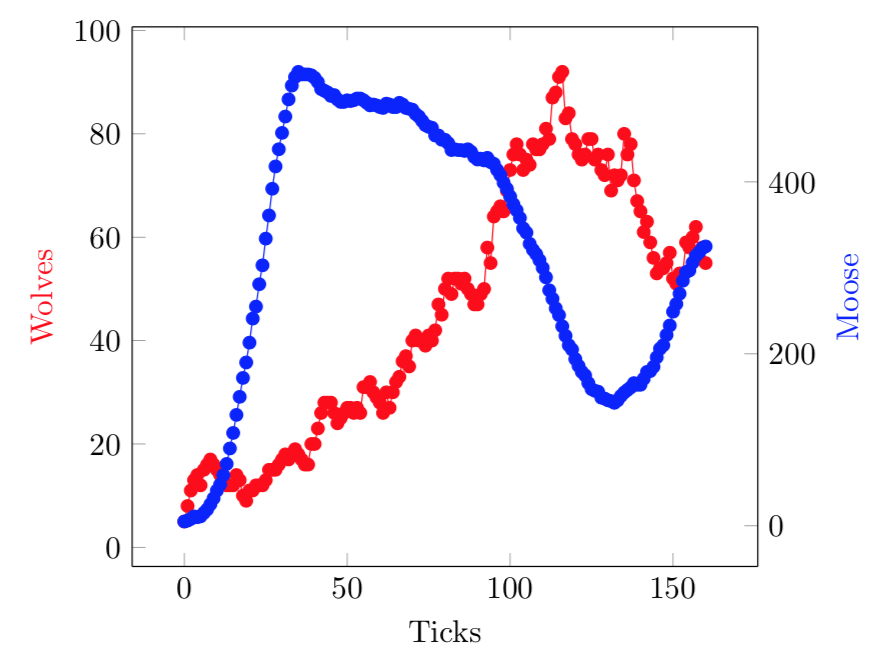
\includegraphics[width=0.60\textwidth]{Experiments/sim_rep_c1}
\caption{Input values: ticks: 150, boardw: 25, moose: 5, moose reproduction length: 4, wolves: 5, wolf reproduction length: 3, wolf hunger length: 4}
\end{figure}

If we change the reproduction length only by one, we see that the number of moose becomes even more, but the opposite can be said for wolves. It takes longer for them to increase significantly, but when they do, again we see that the number of moose decreases. 


\begin{figure}[H]
\centering
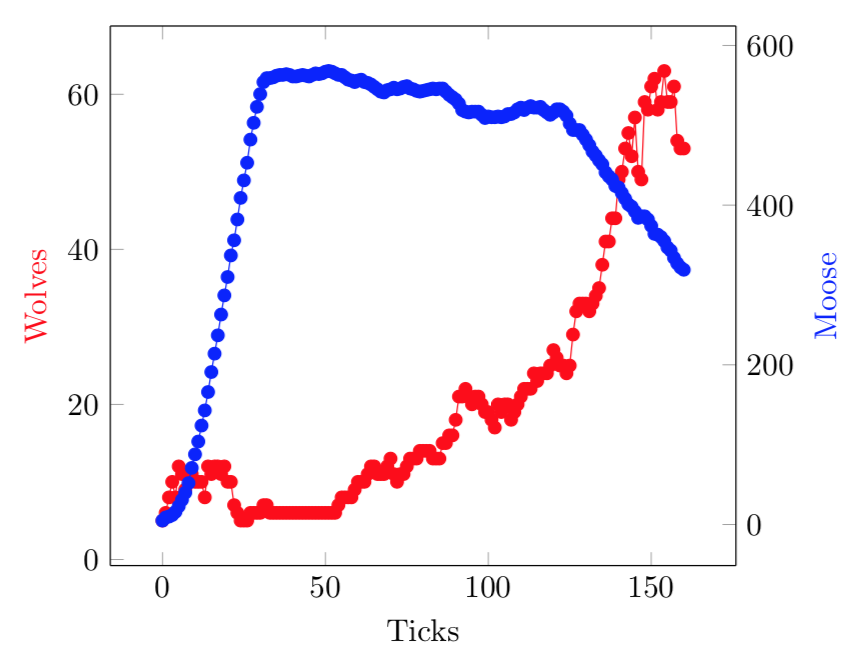
\includegraphics[width=0.60\textwidth]{Experiments/sim_rep_c2}
\caption{Input values: ticks: 160, boardw: 25, moose: 5, moose rep-length: 3, wolves: 5, wolf rep-length: 4, wolf hunger length: 4}
\end{figure}

\subsection*{Conclusion and discussion}
We solved the problem, and programmed the environment to mimic the real world to a certain degree. It is obviously difficult to represent a complicated environment with only a handful of parameters, but the representation that we have build is has many similarities to the environment. There is a clear correlation between the two population of animals.
To improve the representation we could have included the other animals in the environment, the seasons, improved the interaction between the wolf and the moose, and considered that the wolf is a social animal. Another aspect that we could have considered would be that of the breeding season and that a moose usually get one calf while the wolf tends to get several cubs.

\newpage
\section*{Appendix}

\subsection*{User manual}
The application of the Isle Royale is designed to take certain values to initialize the simulation of the wolf and moose population. Specifically the application takes 7 parameters and one file name designed to be given in the following order:
\begin{enumerate}
\item Amount of ticks the users wishes to simulate
\item The file name used for the file the application creates to hold the population data of the current simulation. NOTE: the application automatically applies the file type .csv to the data file. Therefore the users should only insert a title leaving out any white spaces and any typesetting symbols using only casing to indicated word separation. E.g. “IsleRoyale”.
\item Width of the application board
\item Initial population size of moose
\item Length of moose reproduction time measured in number of ticks it takes for a moose to reproduce
\item Initial population size of wolves
\item Length of wolf reproduction time measured in number of ticks it takes for a wolf to reproduce
\item Length of wolf hunger measured in number of ticks a wolf can survive without food
\end{enumerate}

If the user chooses to not apply any values when running the application, the default simulation parameters and file name is set to: mono testIsleRoyale.exe 40 Pop\_IsleRoyale 10 30 10 2 10 4.

To run the application through the console do the following:

\begin{itemize}
\item  Compile the application library by running the following in the terminal/command prompt: fsharpc -a animalsSmall.fsi animalsSmall.fs
\item Next compile the .dll and .fsx file by running the following in the terminal/command prompt: fsharpc -r animalsSmall.dll simulateIsleRoyale.fsx
\item Finally run the application by issuing the following in the terminal/command prompt: mono simulateIsleRoyale.exe either with or without the self defined application parameters. If the user chooses to not apply any values when running the application, the default simulation parameters and file name is set to: mono simulateIsleRoyale.exe 40 test.txt 10 30 10 2 10 4
\end{itemize}

After running the application with the mono command, the user will find a new local \.csv file in the application folder holding the population data of the most recent simulation of Isle Royale. If the user chose to not give any self defined input values, he/she can create a plot of the simulation data by compiling a \.pdf from the file plot\_isleRoyale.tex.

To create a data plot in .pdf through the console write “pdflatex plot\_isleRoyale.tex” in the terminal/command prompt.

\subsection*{Application code}
\lstset{language=FSharp}
\lstinputlisting{animalsSmall.fs}
\end{document}